% dut_tree.tex -- ONE source, ONE rendered SVG (dut_tree.svg), embedded in ../../systems/index.md.
%
% The DUT alone, the same tree in pysim and at RTL: a device (kernel A behind its slave adaptor), a
% composite kernel C (a memory reader, leaf kernel C1, a memory writer), a memory, the crossbar.  Each block is
% coloured by WHO WRITES IT: you (a kernel: run_iter and its HLS body), Waveflow (framework RTL and
% HLS), or vendor IP.  system_cut.tex is the whole system coloured by build step.
%
% Render: bash render.sh   (MiKTeX pdflatex -> PDF -> dvisvgm --pdf -> SVG)
\documentclass[tikz,border=6pt]{standalone}
\usepackage{tikz}
\usetikzlibrary{arrows.meta,positioning,calc,fit,backgrounds}

% The palette of system_cut.tex (theme-neutral: pale fills, explicit strokes).
\definecolor{youfill}{HTML}{DCE9F7}  \definecolor{youline}{HTML}{2C6FB5}   % you write it
\definecolor{wffill}{HTML}{DFF0D8}   \definecolor{wfline}{HTML}{3C7A2E}    % Waveflow provides it
\definecolor{ipfill}{HTML}{EADCF2}   \definecolor{ipline}{HTML}{7A4A9A}    % vendor IP
\definecolor{dutline}{HTML}{1F3B5C}
\definecolor{devline}{HTML}{555555}
\definecolor{inkgray}{HTML}{444444}

\begin{document}
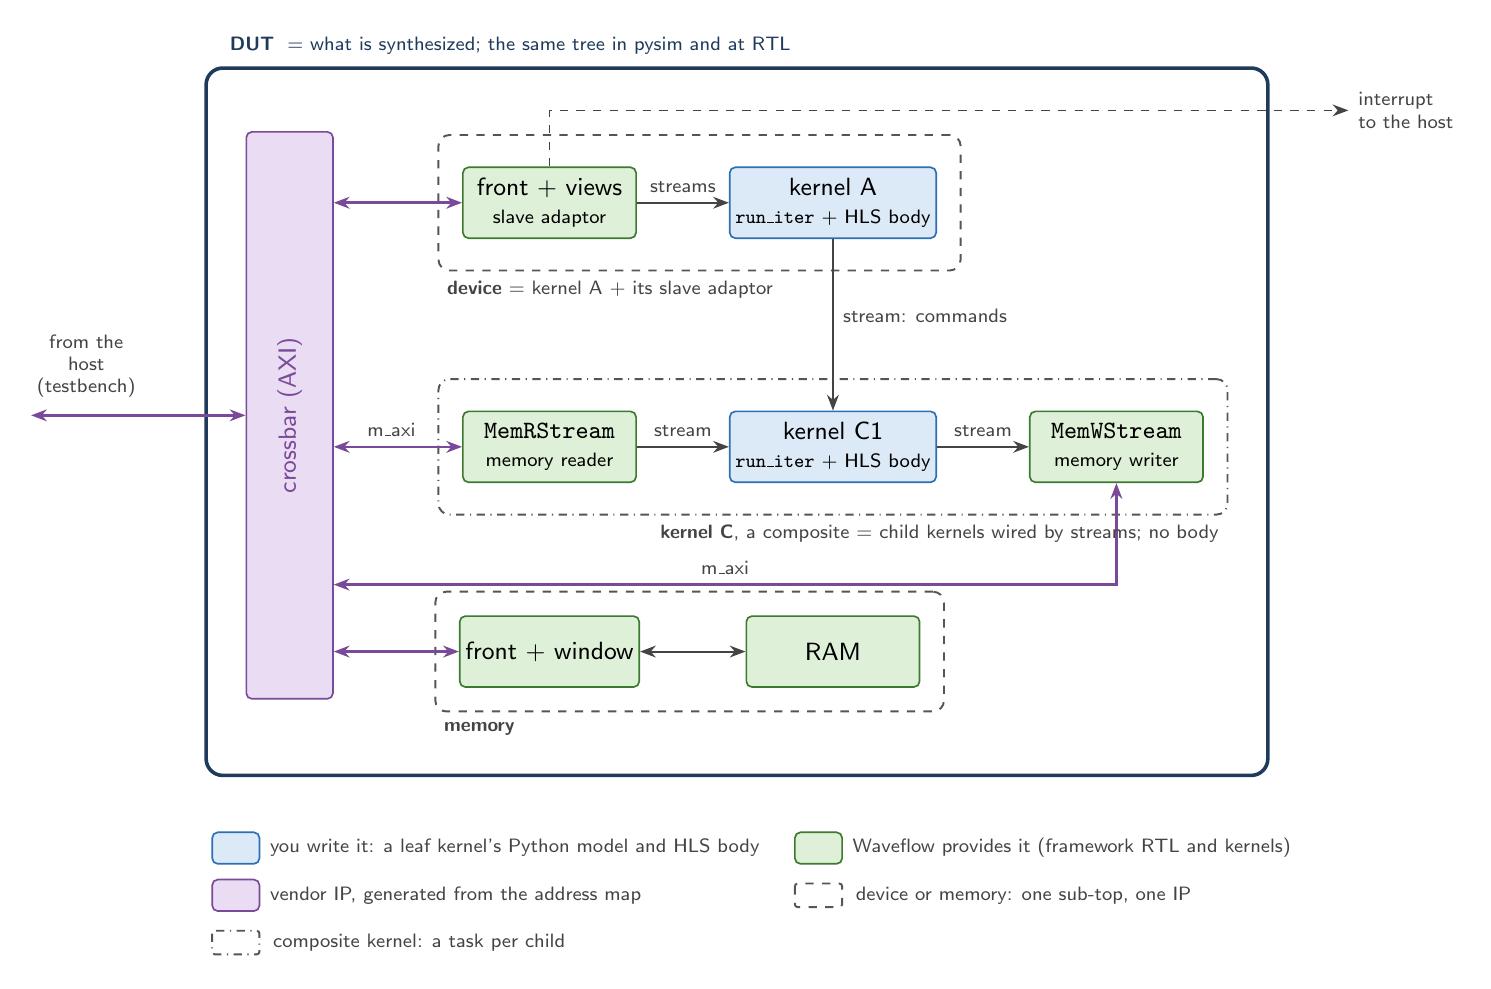
\begin{tikzpicture}[
  font=\sffamily\small,
  blk/.style   = {draw, rounded corners=2pt, minimum height=9mm, align=center, line width=0.6pt,
                  inner sep=2pt},
  you/.style   = {blk, fill=youfill, draw=youline, minimum width=22mm},
  wf/.style    = {blk, fill=wffill, draw=wfline, minimum width=22mm},
  ip/.style    = {blk, fill=ipfill, draw=ipline},
  data/.style  = {-{Stealth[length=2mm]}, line width=0.7pt, draw=inkgray},
  bus/.style   = {{Stealth[length=2mm]}-{Stealth[length=2mm]}, line width=0.9pt, draw=ipline},
  ext/.style   = {-{Stealth[length=2mm]}, line width=0.6pt, draw=inkgray, dashed},
  device/.style= {draw=devline, dashed, rounded corners=4pt, line width=0.7pt},
  comp/.style  = {draw=devline, dash dot, rounded corners=4pt, line width=0.7pt},
  dut/.style   = {draw=dutline, rounded corners=6pt, line width=1.3pt},
  lbl/.style   = {font=\sffamily\scriptsize, text=inkgray},
  tag/.style   = {font=\sffamily\scriptsize\bfseries},
]

% ---------------- the crossbar (vendor IP) ---------------------------------------------------
\node[ip, minimum width=11mm, minimum height=72mm] (xbar) at (0, 0) {};
\node[font=\sffamily\small, rotate=90, text=ipline] at (xbar) {crossbar (AXI)};

% ---------------- the device: slave adaptor + kernel A ---------------------------------------
\node[wf]  (fa) at (3.3, 2.7) {front + views\\[-1pt]\scriptsize slave adaptor};
\node[you] (ka) at (6.9, 2.7) {kernel A\\[-1pt]\scriptsize\texttt{run\_iter} + HLS body};
\draw[data] (fa.east) -- node[lbl, above] {streams} (ka.west);
\draw[bus]  (xbar.east |- fa.west) -- (fa.west);
\begin{scope}[on background layer]
  \node[device, fit=(fa)(ka), inner xsep=3mm, inner ysep=4mm] (dev) {};
\end{scope}
\node[lbl, anchor=north west] at (dev.south west) {\textbf{device} = kernel A + its slave adaptor};

% ---------------- the composite: memory reader -> kernel C -> memory writer ------------------
\node[wf]  (rd) at (3.3, -0.4) {\texttt{MemRStream}\\[-1pt]\scriptsize memory reader};
\node[you] (kc) at (6.9, -0.4) {kernel C1\\[-1pt]\scriptsize\texttt{run\_iter} + HLS body};
\node[wf]  (wr) at (10.5, -0.4) {\texttt{MemWStream}\\[-1pt]\scriptsize memory writer};
\draw[data] (rd.east) -- node[lbl, above] {stream} (kc.west);
\draw[data] (kc.east) -- node[lbl, above] {stream} (wr.west);
\draw[data] (ka.south) -- node[lbl, right, pos=0.45] {stream: commands} (kc.north);
\draw[bus]  (xbar.east |- rd.west) -- node[lbl, above, pos=0.45] {m\_axi} (rd.west);
\begin{scope}[on background layer]
  \node[comp, fit=(rd)(kc)(wr), inner xsep=3mm, inner ysep=4mm] (cmp) {};
\end{scope}
\draw[bus]  (wr.south) |- node[lbl, pos=0.75, above] {m\_axi} (xbar.east |- 0,-2.15);
\node[lbl, anchor=north east] at (cmp.south east) {\textbf{kernel C}, a composite = child kernels wired by streams; no body};

% ---------------- the memory: front + window, RAM --------------------------------------------
\node[wf]  (fm) at (3.3, -3.0) {front + window};
\node[wf]  (rm) at (6.9, -3.0) {RAM};
\draw[data, {Stealth[length=2mm]}-{Stealth[length=2mm]}] (fm.east) -- (rm.west);
\draw[bus]  (xbar.east |- fm.west) -- (fm.west);
\begin{scope}[on background layer]
  \node[device, fit=(fm)(rm), inner xsep=3mm, inner ysep=3mm] (mem) {};
\end{scope}
\node[lbl, anchor=north west] at (mem.south west) {\textbf{memory}};

% ---------------- the DUT ---------------------------------------------------------------------
\begin{scope}[on background layer]
  \node[dut, fit=(xbar)(dev)(cmp)(mem), inner xsep=5mm, inner ysep=8mm] (d) {};
\end{scope}
\node[tag, text=dutline, anchor=south west] at ($(d.north west)+(2mm,0.3mm)$)
     {DUT \;\textmd{= what is synthesized; the same tree in pysim and at RTL}};

% ---------------- the testbench, outside --------------------------------------------------------
\draw[bus] ($(d.west |- xbar.west)+(-2.2,0)$) coordinate (h0) -- (xbar.west);
\node[lbl, align=center, anchor=south] at ($(h0)+(0.7,0.1)$) {from the\\host\\(testbench)};
\coordinate (irq) at ($(fa.north |- dev.north)+(0,0.3)$);
\draw[ext] (fa.north) -- (irq) -- ($(d.east |- irq)+(1.0,0)$)
     node[lbl, right, align=left] {interrupt\\to the host};

% ---------------- legend ---------------------------------------------------------------------
\begin{scope}[shift={($(d.south west)+(0.4,-0.9)$)}, every node/.style={font=\sffamily\scriptsize}]
  \node[you, minimum width=6mm, minimum height=4mm] (l1) at (0,0) {};
  \node[anchor=west, text=inkgray] at (l1.east) {you write it: a leaf kernel's Python model and HLS body};
  \node[wf, minimum width=6mm, minimum height=4mm] (l2) at (7.4,0) {};
  \node[anchor=west, text=inkgray] at (l2.east) {Waveflow provides it (framework RTL and kernels)};
  \node[ip, minimum width=6mm, minimum height=4mm] (l3) at (0,-0.6) {};
  \node[anchor=west, text=inkgray] at (l3.east) {vendor IP, generated from the address map};
  \draw[device, rounded corners=1pt] (7.1,-0.45) rectangle (7.7,-0.75);
  \node[anchor=west, text=inkgray] at (7.75,-0.6) {device or memory: one sub-top, one IP};
  \draw[comp, rounded corners=1pt] (-0.3,-1.05) rectangle (0.3,-1.35);
  \node[anchor=west, text=inkgray] at (0.35,-1.2) {composite kernel: a task per child};
\end{scope}

\end{tikzpicture}
\end{document}
